\documentclass[a4paper,12pt]{article}
\usepackage{graphicx}
\usepackage{amsmath}
\usepackage{geometry}
\usepackage{hyperref}
\usepackage{listings}
\usepackage{color}
\usepackage{tikz}
\usetikzlibrary{shapes.geometric, arrows, positioning}
\usepackage{float} % Ensure figures are precisely positioned with [H]

\geometry{margin=1in}

\title{\textbf{Smart Home Temperature and Humidity Monitoring System}}
\author{Jerin Romijah Tuli \\ 
Roll: 2003056 \\ 
Section: A \\ 
Department of CSE \\ 
Rajshahi University of Engineering and Technology}


% Defining Styles for Block Diagrams
\tikzstyle{block} = [rectangle, draw, text centered, minimum height=2em, minimum width=4em,draw=red, fill=pink!30]
\tikzstyle{arrow} = [thick,->,>=stealth]
\tikzstyle{startstop} = [rectangle, rounded corners, minimum width=3cm, minimum height=1cm, text centered, draw=red, fill=red!30]
\tikzstyle{process} = [rectangle, minimum width=3cm, minimum height=1cm, text centered, draw=blue, fill=blue!10]
\tikzstyle{decision} = [diamond, minimum width=3cm, minimum height=1cm, text centered, draw=green, fill=green!10]

\begin{document}

\maketitle

\begin{abstract}
 This article describes a **Smart House System** intended to control the levels of temperature and humidity. The system makes use of sensors to collect data on the environment, which is displayed on an LCD. Apart from that, it switches on or off home devices like heaters or air conditioners based on the programmed limits. In addition, it is possible to view the information through the smartphone application owing to the Wi-Fi module. This way of life offers both comfort and enjoyable activities; however, there are still some issues to be dealt with, such as calibration of the sensors and reliability of communications.
\end{abstract}

\section{Objectives}
The objectives of the project include the following: 
\begin{itemize}
    \item To continuously monitor the ambient temperature and humidity levels.
    \item To present the measurements in real time, on an LCD display.
    \item To develop a mode of control and supervision via a smartphone.
    \item To control the operation of appliances such as heater or air conditioner by setting up the temperature limits.
    \item To maintain effective coordination between the parts and guarantee that there is no hitch in the hardware and software working together.
\end{itemize}

\section{Scope of the Project}
This system mainly concentrates on climate control in indoor areas and how it can be automated. It measures temperature and humidity values and shows them on the screen and operates the devices when needed. Besides, the users can be able to operate and monitor the system via a smartphone application which is connected to the system through Wi-Fi. Nevertheless, this project addresses only the issue of environmental control and does not go further with more complex solutions such as voice command operability or predictive behavioural analytics.

\section{Block Diagram}
\begin{figure}[H]
\centering
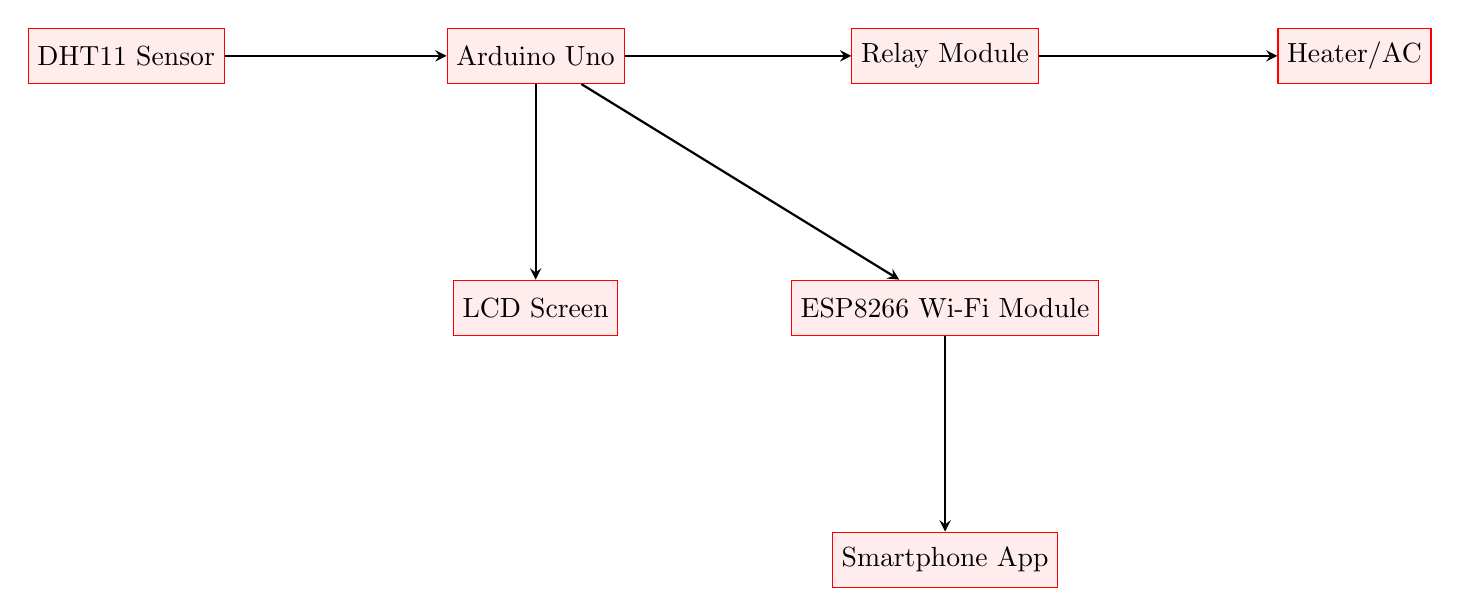
\begin{tikzpicture}[node distance=0.2cm]

% Nodes for Block Diagram
\node (sensor) [block] {DHT11 Sensor};
\node (microcontroller) [block, right of=sensor, xshift=5cm] {Arduino Uno};
\node (lcd) [block, below of=microcontroller, yshift=-3cm] {LCD Screen};
\node (relay) [block, right of=microcontroller, xshift=5cm] {Relay Module};
\node (wifi) [block, below of=relay, yshift=-3cm] {ESP8266 Wi-Fi Module};
\node (appliances) [block, right of=relay, xshift=5cm] {Heater/AC};
\node (app) [block, below of=wifi, yshift=-3cm] {Smartphone App};

% Arrows Connecting Components
\draw[arrow] (sensor) -- (microcontroller);       
\draw[arrow] (microcontroller) -- (lcd);          
\draw[arrow] (microcontroller) -- (relay);        
\draw[arrow] (relay) -- (appliances);             
\draw[arrow] (microcontroller) -- (wifi);         
\draw[arrow] (wifi) -- (app);

\end{tikzpicture}
\caption{Block Diagram of the Smart Home System}
\label{fig:block-diagram}
\end{figure}

\section{Hardware Components}
The essential components which are incorporated in this project are:
\begin{itemize}
    \item \textbf{Arduino Uno:} The basic unit which receives signals from sensors and sends signals to the appliances which are connected to it.
    \item \textbf{DHT11 Sensor:} A device to detect humidity and temperature.
    \item \textbf{LCD Screen:}Used to show data on the spot.
    \item \textbf{Relay Module:}  regulates the on-off cycle of the devices under the feedback from Arduino.
    \item \textbf{ESP8266 Wi-Fi Module:} used for app communication to the cloud over the internet.
    \item \textbf{Power Supply:}  Supplies power to various elements.
\end{itemize}

\section{Software Requirements}
\begin{itemize}
    \item \textbf{Arduino IDE:} It is Application software which is used to develop the applications for Arduino Boards and upload the Programs to the Board.
    \item \textbf{ESP8266 Library:} Responsible for any kind of communication (and internal data management) over the wireless connection.
    \item \textbf{Control Logic:}  Program Logic that controls and operates the appliances when the environmental conditions prescribed are exceeded.
    \item \textbf{User Interface:} A mobile application for controlling and observing the system from a distance.
\end{itemize}

\section{Flowchart of Control Logic}
\begin{figure}[H]
\centering
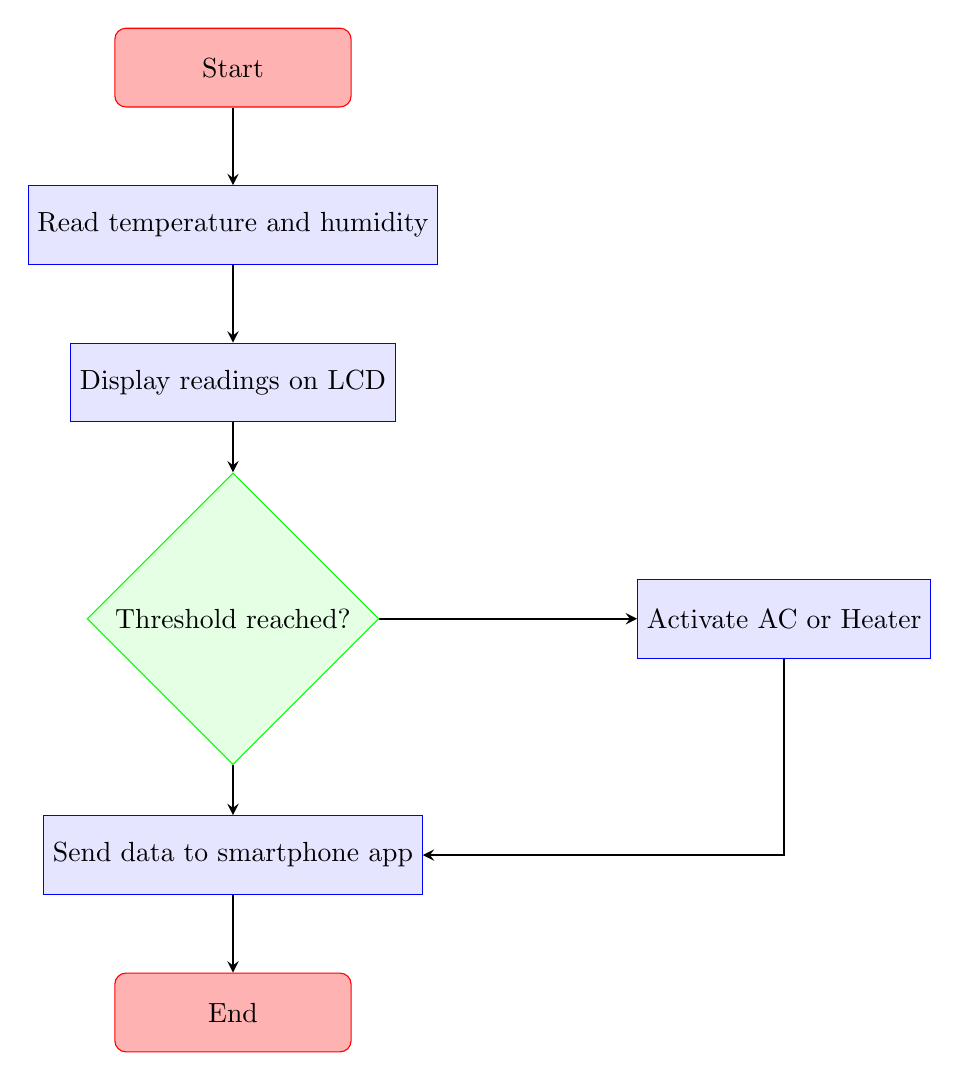
\begin{tikzpicture}[node distance=2cm]

% Nodes for Flowchart
\node (start) [startstop] {Start};
\node (read) [process, below of=start] {Read temperature and humidity};
\node (display) [process, below of=read] {Display readings on LCD};
\node (check) [decision, below of=display, yshift=-1cm] {Threshold reached?};
\node (turnon) [process, right of=check, xshift=5cm] {Activate AC or Heater};
\node (wait) [process, below of=check, yshift=-1cm] {Send data to smartphone app};
\node (stop) [startstop, below of=wait] {End};

% Connecting the Nodes with Arrows
\draw [arrow] (start) -- (read);
\draw [arrow] (read) -- (display);
\draw [arrow] (display) -- (check);
\draw [arrow] (check.east) -- ++(0.5,0) |- (turnon);
\draw [arrow] (turnon) |- (wait);
\draw [arrow] (check.south) -- ++(0,0) -- (wait.north);
\draw [arrow] (wait) -- (stop);

\end{tikzpicture}
\caption{Flowchart of the Control Logic}
\label{fig:flowchart}
\end{figure}

\section{Communication Protocols}
\begin{itemize}
    \item \textbf{I2C:} An Inter Integrated Circuit communication protocol prevents digital noise when sending data to the Arduino and the LCD.
    \item \textbf{UART:} A protocol implemented for wireless communication between the microcontroller and the 8266 WiFi module.
    \item \textbf{HTTP:} A protocol used to send the data that is accommodated in the Wi-Fi module to the mobile app.
\end{itemize}

\section{Hardware-Software Integration}
Arduino Uno interfaces DHT11 sensor to obtain environmental data and displays it on a LCD screen. If the readings of the sensors are above certain limits then the relay module takes care of switching the AC or heater as necessary. The Wi-Fi module works in parallel transmitting the data to a mobile application whereby the users are able to control and monitor the system from a distance.
\section{Data Flow Summary}
\begin{itemize}
    \item **Sensor Data:** The temperature and humidity are gotten from the DHT11 sensor.
    \item **Processing:** The Arduino checks if the readings go above certain set limits.
    \item **Appliance Control:** The relay board controls the appliances in the required manner.
    \item **Display:** The LCD Screen relay’s real-time information to the users.
    \item **Remote Access:** The module wirelessly transmits the information for smartphone application use.
\end{itemize}

\section{Future Enhancements}
\begin{itemize}
    \item Use more monitors including CO2 monitor for enhanced air quality management.
    \item Incorporate systems to facilitate control by voice over Google Assistant and Alexa.
    \item Take creation of smartphone applications a notch higher by including the data in real time graphs.
    \item Use prediction algorithms in climate control for effective utilization of the system.
\end{itemize}

\section{Conclusion}
All in all, this system provides a great alternative for the maintenance of suitable conditions, relative humidities as well as temperatures within an indoor space. It effectively interlinks sensors, wi-fi modules, and relays enables both local operation of devices and operation from a distance. – With enhancements in place, the system might be taken a step further where additional features, for instance, voice management systems or predictive analytics could be integrated.

\end{document}
